\documentclass[a4paper,12pt,oneside]{report}
\usepackage{natbib}         % Pour la bibliographie
\usepackage{url}            % Pour citer les adresses web
\usepackage[T1]{fontenc}    % Encodage des accents
\usepackage[utf8]{inputenc} % Lui aussi
\usepackage[french]{babel} % Pour la traduction française
\usepackage{numprint}       % Histoire que les chiffres soient bien
\usepackage{fancyhdr}

\usepackage{amsmath}        % La base pour les maths
\usepackage{mathrsfs}       % Quelques symboles supplémentaires
\usepackage{amssymb}        % encore des symboles.
\usepackage{amsfonts}       % Des fontes, eg pour \mathbb.
\usepackage{setspace}
\usepackage[svgnames]{xcolor} % De la couleur
\usepackage{geometry}       % Gérer correctement la taille

%%% Si jamais vous voulez changer de police: décommentez les trois
%\usepackage{tgpagella}
%\usepackage{tgadventor}
%\usepackage{inconsolata}


\usepackage{graphicx} % inclusion des graphiques
\usepackage{wrapfig}  % Dessins dans le texte.

\usepackage{tikz}     % Un package pour les dessins (utilisé pour l'environnement {code})
\usepackage[framemethod=TikZ]{mdframed}
% Un environnement pour bien présenter le code informatique
\newenvironment{code}{%
\begin{mdframed}[linecolor=Green,innerrightmargin=30pt,innerleftmargin=30pt,
backgroundcolor=Black!5,
skipabove=10pt,skipbelow=10pt,roundcorner=5pt,
splitbottomskip=6pt,splittopskip=12pt]
}{%
\end{mdframed}
}

%\setmarginsrb{3 cm}{2.5 cm}{3 cm}{2.5 cm}{1 cm}{1.5 cm}{1 cm}{1.5 cm}
\graphicspath{{figures/}}

\title{Rapport de Stage Master 2}
\author{ABAK-KALI Nizar}
\date{\today}

\newcommand{\reporttitle}{Rapport de stage M2}
\newcommand{\reportauthora}{Nizar ABAK-KALI {11290569}} % Auteur
\newcommand{\reportsubject}{} % Sujet
\newcommand{\HRule}{\rule{\linewidth}{0.5mm}}
\setlength{\parskip}{1ex} % Espace entre les paragraphes
\makeatletter
\let\thetitle\@title
\let\theauthor\@author
\let\thedate\@date
\makeatother

\pagestyle{fancy}
\fancyhf{}
\rhead{\theauthor}
\lhead{\thetitle}
\cfoot{\thepage}
\lfoot{
  
\includegraphics [width=20mm]{figures/logop8.jpg}
  }
\rfoot{
  
\includegraphics [width=30mm]{figures/logo_Smile.png}
}
%\renewcommand{\footrulewidth}{1pt}


\begin{document}

%%%%%%%%%%%%%%%%%%%%%%%%%%%%%%%%%%%%%%%%%%%%%%%%%%%%%%%%%%%%%%%%%%%%%%%%%%%%%%%%%%%%%%%%
\begin{titlepage}

\begin{center}

\begin{minipage}[t]{0.48\textwidth}
  \begin{flushleft}
   
\includegraphics [width=30mm]{figures/logop8.jpg} \\[0.5cm]
    \begin{spacing}{1.5}
      %\textsc{Université Paris 8}
    \end{spacing}
  \end{flushleft}
\end{minipage}
\begin{minipage}[t]{0.48\textwidth}
  \begin{flushright}
    
\includegraphics [width=50mm]{figures/logo_Smile.png} \\[0.5cm]
    %\textsc{Neo-Robotix}
  \end{flushright}
\end{minipage} \\[1.5cm]

%\textsc{\Large \reportsubject}\\[0.5cm]
\HRule \\[0.4cm]
{\huge \bfseries \reporttitle}\\[0.4cm]
\HRule \\[1.5cm]

\begin{minipage}[b]{0.3\textwidth}
  \begin{flushleft} \large
    \emph{Auteurs :}\\
    \reportauthora\\
  \end{flushleft}
\end{minipage}
\begin{minipage}[b]{0.6\textwidth}
  \begin{flushright} \large
    \emph{Tuteur :} \\
    M.~Benoit \textsc{COURTY} \\
	M.~Jean Luc \textsc{COSSI} \\
   \end{flushright}
\end{minipage}

\vfill

{\large \today}

\end{center}

\end{titlepage}

\chapter*{Résumé du stage}
Ce stage s'est déroulé dans la société de services Smile et plus particulièrement le département Smile ECS, responsable de l'offre embarqué et IoT\footnote{IoT: Internet of Things ou objets connectés}. Ainsi, mon stage s'est d'abord déroulé sous la tutelle de Pierre Lamot, expert en traitement d'images et streaming chez Smile ECS, puis sous celle de Fabien Dutuit, expert traitement de signal.
\\
Au cours de ce stage, j'ai eu l'opportunité de travailler sur une grande variété de technologies et ainsi d'avoir la chance de pouvoir engranger un maximum de connaissances et d'expériences dans le monde de l'embarqué que je compte utiliser plus tard.
\newline
\newline
Ce stage se découpe en deux phases. Un premier concentré sur l'étude du protocole MPEG-TS ainsi que de son implémentation dans Gstreamer\footnote{\ref{gstreamer}} puis de l'écriture d'un patch décri plus tard dans le rapport, permettant le multiplexage de données non typé dans un flux vidéo. Puis dans un second temps, mon stage c'est plus concentré sur le projet SisselBox\footnote{\ref{sisselbox}}, où je devais dans un premier temps mettre à jour le système de provisionnement, puis implémenter une application afin de tester mon patch.

%%%%%%%%%%%%%%%%%%%%%%%%%%%%%%%%%%%%%%%%%%%%%%%%%%%%%%%%%%%%%%%%%%%%%%%%%%%%%%%%%%%%%%%%%
\tableofcontents
%%%%%%%%%%%%%%%%%%%%%%%%%%%%%%%%%%%%%%%%%%%%%%%%%%%%%%%%%%%%%%%%%%%%%%%%%%%%%%%%%%%%%%%%%
\listoffigures
\pagebreak
%%%%%%%%%%%%%%%%%%%%%%%%%%%%%%%%%%%%%%%%%%%%%%%%%%%%%%%%%%%%%%%%%%%%%%%%%%%%%%%%%%%%%%%%%
\section{Remerciements}
remercier :
  - ECS
  - Pierre
  - Fabien
  - l'equipe ECS
  - Rapotor Jesus
  


\section{Introduction}



-> Pourquoi ce stage, où il s'est déroulé ....



\chapter{Présentation de l'entreprise}

\section{Smile}

Fondé en 1991, Smile est devenu dès 1995 un acteur du web réputé, maîtrisant l’architecture,
les technologies et les outils qui permettent de construire les plus grandes plateformes de
l’Internet.
Depuis 2001, Smile est intégrateur de solutions open source, c'est-à-dire que le cœur de
métier de Smile est la construction de systèmes d’information et de plateformes web
intégrant les meilleures solutions open source du marché.
Smile mène une forte action de veille afin d’identifier les solutions open source les plus
matures et les plus pérennes, qui apporteront un réel bénéfice de compétitivité pour les
entreprises. Smile met à disposition un échantillon de cette expertise au travers de livres
blancs, librement diffusés, qui sont devenus des références dans leurs domaines.
Premier intégrateur spécialisé sur les solutions open source, Smile a été choisi à de
nombreuses reprises par les plus grandes entreprises et administrations pour déployer ces
solutions dans le cadre de projets stratégiques.
Autour du cœur de métier qu’est l’ingénierie, Smile propose une palette de services étendue,
qui lui permet de prendre en charge un projet dans sa globalité : consulting en amont et en
accompagnement des projets, agence interactive intervenant tant en création et
webdesign qu’en conseils éditoriaux, stratégiques et e-marketing, tierce-maintenance
applicative (TMA), formation, support et maintien en conditions opérationnelles, et enfin
hébergement et exploitation.
Smile possède également un rayonnement international grâce à ses dix-sept agences
réparties dans 9 pays.

\begin{figure}[!h]
  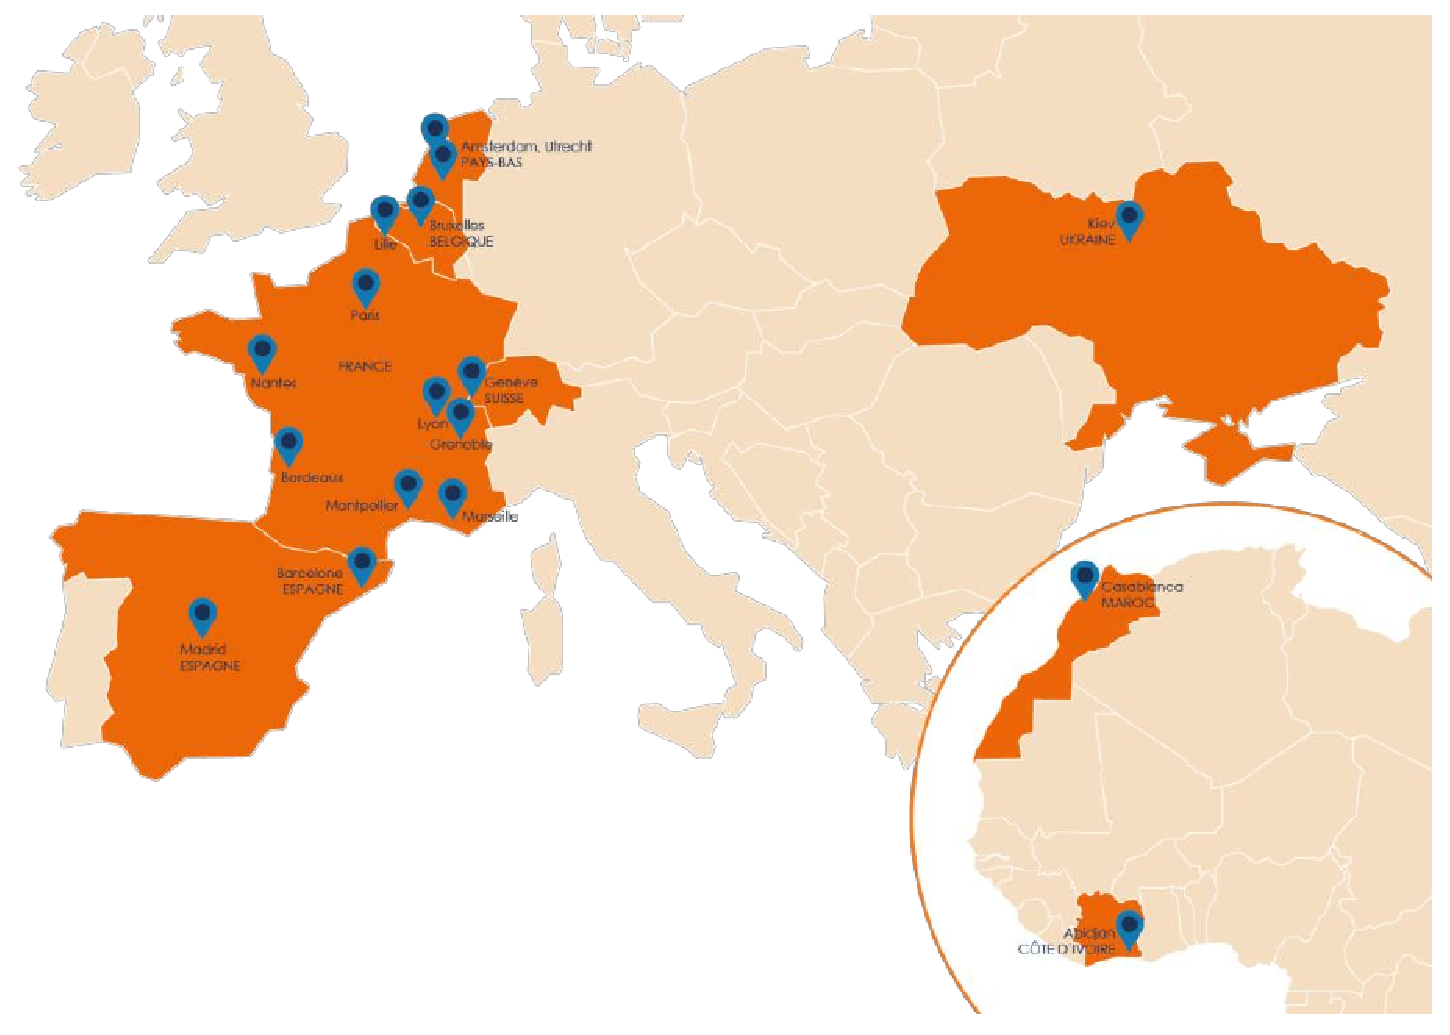
\includegraphics[scale=0.7]{carte_smile}
  \caption{\label{smile_map} Agences Smile}
\end{figure}

Smile organise également une veille technologiques importantes sur l’open source, avec la
rédaction de nombreux livres blancs par les différents consultants sur des sujets variés allant
des solutions web d’e-commerce, en passant par les middlewares et finissant par
l’embarqué. Il existe actuellement une vingtaine de livres blancs, renouvelés tous les 2-3 ans
pour inclure les nouveautés des différentes technologies.
Dès 2001, Smile commence à construire son expertise des solutions open source : un choix
d’avenir que beaucoup de ses concurrents n’osent pas alors entreprendre.
A partir de 2004, les grandes entreprises adoptent de plus en plus souvent les solutions open
source. Smile occupe une position solide de leader sur ce marché qui décolle, élargissant
progressivement son offre vers de nouveaux domaines – CMS, Portails, e-Commerce,
Décisionnel, Infrastructure, ERP - et créant des services associés : agence média, tierce
maintenance, exploitation, système. En 2007, Smile affiche plus de 50\% de croissance et
inaugure trois nouvelles agences à Lyon, Nantes et Bordeaux.
En 2008, Smile compte plus de 270 collaborateurs et poursuit sa croissance en se
développant à l'international, notamment à Kiev en Ukraine.
En 2009, Smile compte 320 collaborateurs dans le monde et poursuit son extension
internationale. En juin 2009, Smile intègre Cometa Technologies S.L., basée à Barcelone et
compte alors 8 agences dans le monde.
En 2011, Smile regroupe 500 collaborateurs et ouvre ses agences à Bruxelles, Utrecht et
Amsterdam.

En 2013, Smile compte 700 collaborateurs et 17 agences.
2014 est une année importante pour Smile, avec plus de 20\% de croissance sur ces cinq
dernières années et près de 700 collaborateurs dans le monde. Au fil de ces années, Smile est
devenu un acteur incontournable de l’open source, leader en France et en Europe.
En 2015, Smile annonce être en négociations exclusives avec la société Open Wide en vue
d’un rapprochement. Ceci afin d'élargir son offre et renforcer son leadership.


\section{Smile ECS}
Smile ECS, ex-OpenWide est une société spécialisée dans le domaine de l'open source, racheté par Smile. J'ai décidé d'intégrer cette entreprise pour mon projet de fin d'étude à l'université Paris 8 afin
d'approfondir mes connaissances dans le domaine du logiciel libre, et celui de l'embarqué.
 Les technologies Open source devenant de plus en plus prédominantes dans la paysage informatique
moderne, intégrer une société spécialisée dans cette technologie était une façon pour
moi de donner un cap sur l'orientation de ma carrière professionnelle.
Ce rapport explicitera mon travail durant ce stage de fin d'étude, qui a duré
six mois, dont le sujet a été d'améliorer le système de transmission des données,
afin de pouvoir transmettre un flux vidéo, de caméras de sécurité, avec des métadonnées
calculées depuis ce flux (exemple: positions des visages détectés). Puis dans un second temps,
recupérer ce flux afin de le stocker pour un visionnage ultérieur.
Après une explication du cadre du stage, j'essaierai de développer les technologies
utilisées lors de ce stage.

\newpage
\section{Présentation du sujet}
Mon sujet s'inscrit dans un projet developpé en interne, le projet SisellBox. Ansi,
je vais présenter dans un premier temps le projet, puis dans un second temps
expliquer ou je m'inscrit dans le projet et qu'est ce que j'y apporte.

\subsection{Le projet SisellBox}
  \subsubsection{ça fait quoi}
  \subsubsection{pour qui}
  \subsubsection{Architecture du projet (Schéma + commentaire)}
  $\rightarrow$ schema general de la sBox
  \begin{itemize}
    \item Sbox Streamer
    \item Sbox Recorder
  \end{itemize}

\subsection{La problématique posé}
\begin{itemize}
  \item Etude de Gstreamer
  \item Etude du protocole MPEG-TS
  \item Transmission de flux vidéo + métadonnée
  \item patch du plugin Gstreamer mpegtsmux afin de  multipler les donnes
  \item patch du plugin de Gstreamer mpegtsdemux afin demultplexer les données pour le stockage
  \item afficher les metadonnée sur une une interface a
\end{itemize}

\newpage
\chapter{Présentation de l'environnement de travail}
Dans le cadre de se stage j'ai eu l'occasion de travailler une plusieurs technologie, beaucoup d'entre-elles m'était inconnue. Ainsi , je vais explicité les différentes technologie sur lesquelles j'ai travailler.
\section{Configuration}
\section{Gstreamer}
\label{gstreamer}
\section{OpenCV}
\section{Protobuf et Grpc}
\section{Outils de provisionnement}

\newpage
\chapter{Travail réalisé}
Dans ce chapitre je décrirai les tâches accomplies lors de ce stage, ainsi que les difficultés rencontrées.
\section{Modifications du plugin Gstreamer MPEG-TS}
% Pourquoi
Comme expliqué précédemment, mon stage s’inscrit dans une continuité, et donc a pour but d'améliorer le système déjà présent. Avant ma participation au projet, le système prenait des flux vidéo de sources différentes (caméras de sécurité, fichier vidéo, etc.), pour ensuite faire passer ce flux vidéo par des briques algorithmiques de traitement d'images (détection des visages, détection de mouvement...). De ce traitement d'images on extrait des métadonnées, dans le cas de la détection de visages nous obtenons des rectangles représentant la surface recouvrants les visages. Ces métadonnées étaient formatées au format ONVIF\footnote{ONVIF où "Open Network video interface Forum" est une convention internationale, qui a pour but de faciliter le développement du standard pour l'interfaçage des produits de sécurité avec adresse IP, exemple caméra de sécurité}. Le flux vidéo et le flux de métadonnées sont "temporisées", afin qu'ils soient synchronisés plus tard, puis ils sont ajoutés au conteneur MKV\footnote{le format MKV (Matroska Video) est un format vidéo entièrement libre. Plus exactement il s'agit d'un conteneur (d'où le nom Matroska, en référence aux poupées russes) permettant de contenir de la vidéo (Divx, Xvid, RV9, etc.), du son (MP3, Ogg, MP2, AC3, DTS, AAC, PCM), ainsi que des sous-titres (SRT, ASS, SSA, USF, etc.) dans un même fichier.} pour la transmission. Ainsi, le flux de métadonnées était passé en sous-titres dans le fichier MKV. Or, le format MKV recevait les métadonnées formatées au format ONVIF (sous forme XML), il reformatait de nouveau ce flux, ce qui corrompait les métadonnées. C'est de cette problématique que découle mon stage, on avait besoin de transmettre le flux vidéo/métadonnées au travers d'un protocole standard sans avoir modifié le format des métadonnées. Ainsi nous nous sommes intéressés au protocole MPEG-TS.
% qu'est c'est

\subsection{Architecture de MPEG-TS}
MPEG-TS ou MPEG Transport Stream permet de contenir du flux digital (audio, vidéo, ou bien privé tel que des sous-titres). Il intègre aussi la synchronisation de flux et la correction  d'erreur lors d'une perte de paquet. L'autre intérêt de MPEG-TS est qu'il peut contenir plusieurs "programmes" dans un flux. Chaque programme peut contenir N flux vidéo ou audio ou privés. Chacun de ces flux à un identifiant ou "PID"\footnote{Packet ID} et chaque programme a un PID\footnote{dans ce cas si PID veut dire Program ID}. Les programmes sont enregistrés dans une PMT\footnote{Programme Map table} une table des programmes regroupant les différents programmes. Les PMT sont ensuite enregistrés dans une PAT\footnote{Programme Association table}.

\begin{figure}[!h]
  \centering
  \includegraphics[scale=0.7]{figures/ts_diag}
  \caption{schéma de l'encapsulation de média dans MPEG-TS}
\end{figure}

\begin{figure}[!h]
  \centering
  \includegraphics[scale=0.6]{figures/ts}
  \caption{schéma d'une trame d'une section Transport Stream}
\end{figure}

\subsection{Explication des plugins mpegtsmux et tsdemux}
% qu'est ce que j'ai fait ?
Suite à l'étude de MPEG-TS au niveau architecturale, je me suis mis à étudier et à comprendre le code de l'implémentation sous Gstreamer. L'implémentation se compose en deux partie,
la partie "multiplexage",et la partie "démultiplexage". Comme presque tout les plugins, elle sont codés en C avec la librairie GObject\footnote{GObject est une interface de programmation et une bibliothèque logicielle multiplateformes publiée sous licence libre (LGPL), qui permet de manipuler des objets, ainsi que d'avoir accès à une palette d'objets élémentaires. Deplus, GObject s'interface très bien avec d'autres langages de programmation comme Python ou bien Vala.}.\\
  \paragraph{Le plugin mpegtsmux}
Le multiplexage se fait au travers du plugin \textbf{mpegtsmux}. Le flux de données entre depuis le pad d'entrée\footnote{cf. \ref{principe gst}} avec une négociation des caps qui donne le type multimédia du flux (exemple : vidéo/x-raw, qui est un flux vidéo pur sans encodage) puis le flux est découpé en paquets "temporisés", et identifiés. Tout les flux sont traités de cette manière. Ensuite tous les paquets sont "entrelacés" dans un seul flux puis mis à disposition sur le pad de sortie.
  \paragraph{Le plugin mpegtsdemux}
Le démultiplexage fonctionne à l'inverse. Les paquets reçus sont analysés par \textbf{tsparse}, plugin qui parse les paquets TS et qui les donne à \textbf{mpegtsdemux} . Ensuite le mpegtsdemux refabrique les différents flux et crée un pad à la demande (ou "request pad" dans la littérature anglophone) par flux. Il suffit donc de se connecter à ces pads de sortie pour avoir le flux que l'on souhaite

\subsection{Modifications apportées au plugins}

\paragraph{Ajout d'un nouveau types élémentaire:} Les plugins permettent de muxer et demuxer du flux multimédia connu, dont le type multimédia à un code\footnote{cf. \url{https://en.wikipedia.org/wiki/Program-specific_information#Elementary_stream_types}}. Or pour des raisons d'interopérabilité avec d'autres plateformes et logiciels nous avons décidé de créer un nouveau type élémentaire dans le code. Ce type est ajouté aux deux plugins \footnote{cf. \ref{tsmux_annexes_h}}.
\paragraph{Modifications du muxer pour accepter le nouveau type:} Après avoir ajouté un nouveau type élémentaire, il faut que lorsque le muxage soit fait, on puisse identifier le flux avec son type et lui donner son ID . Cela est fait en modifiant la méthode \textbf{mpegtsmux\_create\_stream}. Lors de la négociation des caps on récupère le type du flux, ici "application/x-private". Ensuite on test le type et on attribut le l'"element stream type" pour le flux, dans notre cas \textbf{TSMUX\_ST\_PS\_PRIVATE}. Ensuite on attribut le PID du flux, grâce à la méthode de \textbf{tsmux\_create\_stream}, soit en passant un entier de 32 bit, soit la méthode boucle jusqu'à trouvé un PID vacant.
\paragraph{modifications du demuxer:}  Les modifications du démuxer sont plus simples puisqu'il s'agit récupérer un flux de type "application/x-private" puis d'ouvrir un pad de sortie et de fournir le flux demandé . Pour ce faire j'ai ajouté un test dans la méthode "create\_pad\_for\_stream" puis j'ai créé les caps qui convenaient.
\begin{lstlisting}[language=C, caption=création de caps pour le flux sortant,label=demux_c]
...
case DRF_ID_XPRIVATE:
          sparse = TRUE;
          is_private = TRUE;
          caps = gst_caps_new_simple ("application/x-private",
              "parsed", G_TYPE_BOOLEAN, TRUE, NULL);
          break;
...
\end{lstlisting}

Après test j'ai pu transmettre du flux vidéo accompagné de données générer aléatoirement et donc pue passer à la deuxième partie de mon stage .

\section{Projet SisellBox}

Pour la seconde phase de mon stage, il m'a été attribué de modifier et d'automatiser le système de provisionnement du système tournant sur VM. et ensuite de tester les plugins MPEG-TS dans le contexte de projet.

% Pourquoi j'ai Modification + - Sisell elements\\ - sboxstreamer\\
 \subsection{Étude de l'existant}
J'ai dans un premier temps étudié le projet dans son ensemble, voici une description non exhaustive du projet
  \begin{description}
   \item [ansible : ] contient tout ce qui concerne le provisionnement de la machine VM ainsi que la gestion des VMs avec Vagrant.
  \item [dataset : ] contient des vidéos de tests .
  \item [httpproxy : ] contient les configurations du serveur web nginx.
\item [sboxweb : ] contient l'interface web du projet, contenant le backend codé en Python Flaskr.
\item [simple\_stream : ] contient l'application de test que j'ai développée.
\item [sisell\_éléments : ] contient les briques algorithmiques de traitement d'images et interfacé avec Gstreamer sous forme de plugins
  \end{description}

 \subsection{mise à jour du système de provisionnement}
 % a quoi ressemblait l'archi avant puis ce que l'on en fait apres
La nouvelle architecture qui m'a été demandé d'implémenter à pour but de simplifier la compréhension du système de provisionnement mais aussi de simplifier les modifications futures. La découpe est la suivante :
  \begin{description}
   \item [1\_devenv] une brique réservée au provisionnement des outils qui mette en place un environnement de développement
   \item [2 \_streamers] partie installe les outils de développement nécessaires au streamer, principalement les paquets Gstreamer
   \item [3 \_streamers\_dev] rôles qui cherche les sources Gstreamer, les configure, les compile, et enfin fabrique des paquets Debian pour faciliter la gestion de ces paquets
   \item [4\_control] script qui compile et installe toutes sources et librairies qui sont responsables du contrôle au sens le plus abstrait de l'application. On peut y trouver les librairies grpc et Protobuf, ainsi que leurs binders Python.
   \item [5\_algo] brique consacré à l'installation des librairies Open Cv.
  \end{description}

  \begin{lstlisting}[caption=exemple de rôles Ansible ,label=ansible_exemple]
    - name: Install Mysql package
  yum: name={{ item }} state=present
  with_items:
   - mysql-server
   - MySQL-python

- name: Configure SELinux to start mysql on any port
  seboolean: name=mysql_connect_any state=true persistent=yes
  when: sestatus.rc != 0

- name: Create Mysql configuration file
  template: src=my.cnf.j2 dest=/etc/my.cnf
  notify:
  - restart mysql

- name: Start Mysql Service
  service: name=mysqld state=started enabled=yes

- name: Create Application Database
  mysql_db: name={{ dbname }} state=present

- name: Create Application DB User
  mysql_user: name={{ dbuser }} password={{ upassword }}
  \end{lstlisting}


 Ensuite, pour créer une machine virtuelle à l'aide Vagrant et la provisionner, il suffit de taper la commande :
  \begin{lstlisting}[language=bash]
  vagrant up --provision
  \end{lstlisting}
 Une VM est lancée on peut donc y accéder depuis un lien ssh sécurisé que Vagrant fournit :
  \begin{lstlisting}[language=bash]
  vagrant ssh
  \end{lstlisting}


 \subsection{Application de Test}
La finalité de mon stage fut de pouvoir streamer un flux MPEG-TS contenant un flux vidéo, et des métadonnées obtenues depuis des algorithmiques de traitement d'images, au travers du protocole RTP. Ainsi mon but a été de transmettre depuis une VM jusqu'à ma machine.
Voici les pipelines réalisées :

\paragraph{Coté streamer: }

\begin{verbatim}
 GST_DEBUG=3 GST_DEBUG_DUMP_DOT_DIR=./stream \
	 gst-launch-1.0 filesrc location=/dataset/videoMP4.mp4 do-timestamp=true !\
	   decodebin ! video/x-raw,format=I420 ! tee name=src  \
	 mpegtsmux name=m ! video/mpegts ! rtpmp2tpay ! udpsink host=10.1.75.173 port=5555 \
	 src. ! queue name=post_face_queue max-size-time=0 max-size-bytes=0\
	   max-size-buffers=0  ! videoconvert ! video/x-raw,format=BGR ! \
	     owfacedetect name=face !\
	       capssetter caps="application/x-private,parsed=true"\
		 replace=true join=false ! m. \
	 src. ! queue name=video_q  ! x264enc ! m.
\end{verbatim}
La pipeline ci-dessus est celle qui se charge de streamer. On peut lire les variables GST\_DEBUG et GST\_DEBUG\_DUMP\_DOT\_DIR qui sont utiles pour avoir des logs plus verbeux et indiqués où l'on veut que les graphes ".dot" soit générés. Le plugin \textbf{filesrc} cherche le fichier MP4, le lit, et le fournit sur son pad de sortie. La propriété "do timestamp" est mise à true afin que le plugin écrive des paquets temporisés. le flux vidéo et ensuite donné à un élément appelé \textbf{decodebin}. Il va se charger de décoder le flux et retourner sur son pad se sortit le type demandé en caps, ici "vidéo/x-raw, format=I420". la vidéo décodée va être récupérée par l'élément \textbf{tee} que l'on nomme "src". Il se charge de dupliquer sur le flux pour autant de branches qui demandent. La prémière fournie est celle-ci reliée au plugin mpegtsmux patché, tandis que la deuxième branche convertit l'encodage des couleurs du flux vidéo d'I420 vers du BGR\footnote{BGR: Blue, Green, Red} pour le plugin de détection owfacedetect. Les métadonnées sont ensuite données, post-négociation de caps, au multiplexeur. Il en va de même pour la vidéo qui est encodée en H.264 par \textbf{x264enc}. Le muxer produit des paquets TS qu'il fournit au plugin \textbf{rtpmp2tpay} qui les empaquette dans des paquets RTP pour ensuite les envoyer par UDP grâce au plugin\textbf{udpsink} .


\paragraph{Coté recoder: }

\begin{verbatim}
  GST_DEBUG=4 GST_DEBUG_DUMP_DOT_DIR=./record \
	 gst-launch-1.0 udpsrc port=5555 ! application/x-rtp,media=video,clock-rate=90000,\
	   encoding-name=MP2T ! rtpmp2tdepay ! tsparse ! tsdemux name=d \
	 d.private_0041 ! queue name=meta_queue ! filesink location=lol\
	 d.video_0042 !  queue name=video_queue ! video/x-h264 ! h264parse ! \
	   avimux ! filesink location=lol.avi  \
\end{verbatim}
Cette pipeline fait l'inverse du streamer . On récupère le flux RTP/TS au travers d'UDP, puis \textbf{rtpmp2tdepay} dés-empaquette les paquets TS. Ces derniers sont analysés par \textbf{tsparse} qui fournit au plugin \textbf{tsdemux} un flux TS à demuxer. Ensuite il suffit de lire les bons pads pour avoir ce que l'on veut. Comme par exemple ci-dessus le flux privé est sur le pad "private\_0041".

\paragraph{Problème de trou dans le flux de métadonnées}
Le principal problème rencontré est la désynchronisation des flux due à un manque de métadonnées, cas qui arrive souvent dans le cas où l'on ne détecte pas de visages. La solution a été de modifier le plugin \textbf{owfacedetect} qui hérite d'une classe mère OWCollectPadData. Cette dernière est une classe générique qui fabrique et gère la vie d'un plugins ainsi que la gestion de pads. Nous avons donc choisit d'hériter d'une classe plus riche, GstBaseTransform qui offre des fonctionnalités innées comme le comblement de vide dans un flux par des Segment. La classe segment sert à signaler que le paquet transmis est vide et combien de temps.
\newpage
\section{Conclusion}
\begin{comment}
(à peu près 1 page)

­ ??? (conclusion du stage)

­ Quelques chose de personnel : ton sentiment, ce que tu en as tiré, ??

­ Ouverture vers la suite :
\end{comment}
\newpage
\include{content/ref}

\end{document}
